%
%	Praxisbezug
%

\pagebreak
\section{mTLS Analysis}

\onehalfspacing

\subsection{Resource Consumption}

To evaluate the two service meshes, we will look at the following Kubernetes metrics:\footnote{See \textit{Kubernetes (2023)}: Resource Pipeline. \cite{resPipeline}}

\begin{itemize}
    \item Number of pods
    \item CPU reserved
    \item CPU used
    \item Memory reserved
    \item Memory used
\end{itemize}

We will take the values from the Rancher cluster dashboard for each experiment iteration.

\begin{figure}[H]
\centering
\caption {Cluster Dashboard}
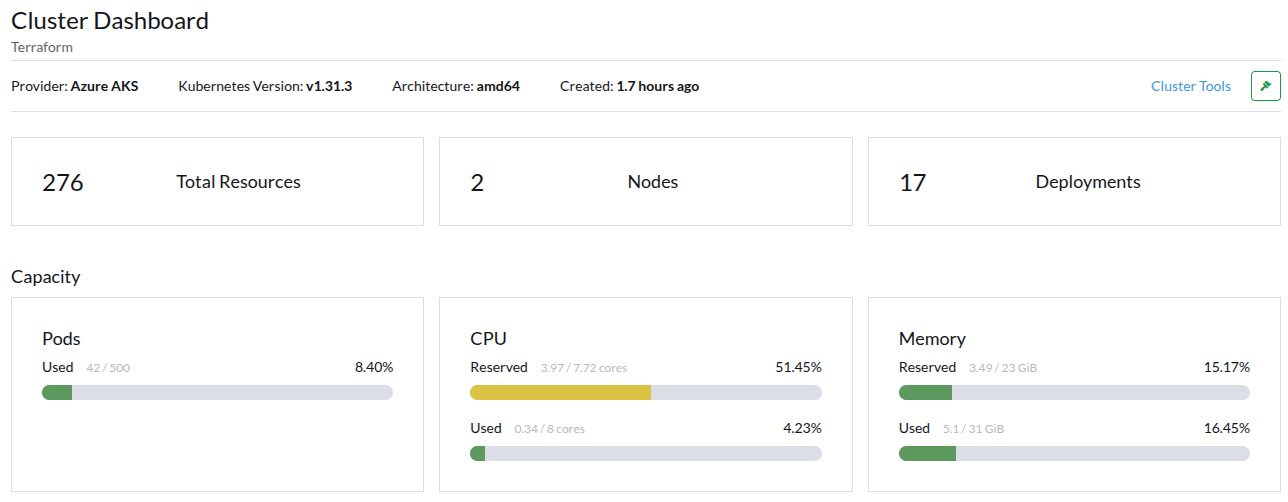
\includegraphics[width=\linewidth]{images/cluster-dashboard.png}
\label{fig:clusterDashboard}
\end{figure}

Here are the tabulated results from the experiment:

\begin{table}[h]
  \centering
  \caption{Resource Consumption}
    \begin{tabular}{| l | l | l | l | l | l |}
    \hline
    & Pods & CPU Rsvd & CPU Used & Memory Rsvd & Memory Used \\
    \hline\hline
    Idle & 37 & 3.97 & 0.32 & 3.49 & 4.78 \\
    \hline
    App Only & 42 & 3.97 & 0.34 & 3.49 & 5.1 \\
    \hline
    \hline
    \end{tabular}
  \label{tab:resUsage}
\end{table}

\subsection{Findings from LinkerD}

\subsection{Findings from Istio}

\subsection{LinkerD and Istio Evaluation}

\subsection{Outlook}
